\subsection{Experimental Results on STR-MF} \label{experimental_results_spatial}
Next we focus on using the Berkeley dataset to verify the STR-MF model as the sensor node location information for the Traffic data is incompletely specified and thus unable to be properly exploited.
\begin{table} [h]
\caption{RMSE of Berkeley, Random Missing and Consecutive Missing} \label{table:spatial}
\tiny
\setlength{\tabcolsep}{1pt}
%\centering
\begin{tabular} {c | r r r | r r r | r r r | r r r | r r r | r r r }
& \multicolumn{9}{ c|}{Random Missing} & \multicolumn{9}{ c }{Consecutive Missing}\\ \hline
& \multicolumn{3}{ c|}{Humidity} & \multicolumn{3}{ c|}{Light} & \multicolumn{3}{ c| }{Temperature} 
& \multicolumn{3}{ c|}{Humidity} & \multicolumn{3}{ c|}{Light} & \multicolumn{3}{ c }{Temperature} \\ \hline
train & \begin{turn}{70}TR-MF\end{turn} & \begin{turn}{70}STR-MF\end{turn} & \begin{turn}{70}sTR-MF\end{turn}& \begin{turn}{70}TR-MF\end{turn} & \begin{turn}{70}STR-MF\end{turn} & \begin{turn}{70}sTR-MF\end{turn}& \begin{turn}{70}TR-MF\end{turn} & \begin{turn}{70}STR-MF\end{turn} & \begin{turn}{70}sTR-MF\end{turn} 
& \begin{turn}{70}TR-MF\end{turn} & \begin{turn}{70}STR-MF\end{turn} & \begin{turn}{70}sTR-MF\end{turn}& \begin{turn}{70}TR-MF\end{turn} & \begin{turn}{70}STR-MF\end{turn} & \begin{turn}{70}sTR-MF\end{turn}& \begin{turn}{70}TR-MF\end{turn} & \begin{turn}{70}STR-MF\end{turn} & \begin{turn}{70}sTR-MF\end{turn} \\ \hline
10\% & $ \mathbf{ 0.142 } $ & $ 0.484 $ & $ 0.173 $ & $ \mathbf{ 35.5 } $ & $ 97.4 $ & $ 38.3 $ & $ \mathbf{ 0.046 } $ & $ 0.154 $ & $ 0.061 $ 
& $ 0.957 $&$ 0.573 $&$ \mathbf{ 0.547 } $&$ \mathbf{ 220.0 } $&$ 281.6 $&$ 264.7 $&$ 0.515 $&$ \mathbf{ 0.242 } $&$ 0.307 $\\
20\% & $ \mathbf{ 0.114 } $ & $ 0.424 $ & $ 0.135 $ & $ \mathbf{ 28.2 } $ & $ 90.6 $ & $ 28.9 $ & $ \mathbf{ 0.032 } $ & $ 0.146 $ & $ 0.047 $ 
& $ 0.796 $&$ 0.657 $&$ \mathbf{ 0.459 } $&$ \mathbf{ 113.3 } $&$ 236.8 $&$ 230.0 $&$ 0.392 $&$ \mathbf{ 0.179 } $&$ 0.187 $\\
40\% & $ \mathbf{ 0.092 } $ & $ 0.352 $ & $ 0.104 $ & $ \mathbf{ 21.2 } $ & $ 85.8 $ & $ 22.8 $ & $ \mathbf{ 0.023 } $ & $ 0.145 $ & $ 0.037 $ 
& $ 0.771 $&$ 0.520 $&$ \mathbf{ 0.455 } $&$ \mathbf{ 58.0 } $  & $ 110.7 $ &  $ 64.3 $&$ 0.310 $&$ 0.196 $&$ \mathbf{ 0.189 } $\\
60\% & $ \mathbf{ 0.082 } $ & $ 0.337 $ & $ 0.093 $ & $ \mathbf{ 17.2 } $ & $ 83.3 $ & $ 18.3 $ & $ \mathbf{ 0.018 } $ & $ 0.147 $ & $ 0.031 $ 
& $ 0.540 $&$ \mathbf{ 0.351 } $&$ 0.708 $&$ \mathbf{ 41.7 } $  & $ 150.1 $ &  $ 69.2 $&$ 0.206 $&$ \mathbf{ 0.191 } $&$ 0.243 $\\
80\% & $ \mathbf{ 0.076 } $ & $ 0.324 $ & $ 0.084 $ & $ \mathbf{ 17.7 } $ & $ 84.4 $ & $ 18.1 $ & $ \mathbf{ 0.015 } $ & $ 0.148 $ & $ 0.027 $ 
& $ 0.447 $&$ 0.299 $&$ \mathbf{ 0.261 } $&$ \mathbf{ 21.4 } $  & $ 112.6 $ &  $ 28.0 $&$ 0.132 $&$ \mathbf{ 0.108 } $&$ 0.114 $\\
85\% & $ \mathbf{ 0.075 } $ & $ 0.326 $ & $ 0.083 $ & $ \mathbf{ 14.4 } $ & $ 82.0 $ & $ 15.8 $ & $ \mathbf{ 0.016 } $ & $ 0.138 $ & $ 0.028 $ 
& $ 0.323 $&$ \mathbf{ 0.166 } $&$ 0.256 $&$ \mathbf{ 8.3 } $   & $ 85.4 $  &  $ 12.0 $&$ 0.088 $&$ \mathbf{ 0.065 } $&$ 0.082 $\\
\end{tabular}
\end{table}
%\vspace{-0.2in}

%Table \ref{table:spatial_random_hum}, \ref{table:spatial_random_light}, \ref{table:spatial_random_tem}, \ref{table:spatial_temporal_hum}, \ref{table:spatial_temporal_light}, \ref{table:spatial_temporal_tem}  show the result of adding spatial regularization.

Tables~\ref{table:spatial} compare STR-MF with TR-MF.
The spatial regularization used for STR-MF was defined based on manually-determined neighborhood nodes established via inspection of the floor plan, as shown in Figure \ref{fig:expected_similarity}.
Note that STR-MF and sTR-MF stand for TR-MF with strong and relatively weaker spatial regularization, respectively.
The results show that for the random missing pattern, adding spatial regularization indeed hurts the performance.
We believe this perhaps surprising finding holds for the random missing cases because the sensor observations alone are adequate for TR-MF to learn the correlations between sensors, hence enforcing similarity between nearby sensors can actually degrade accuracy because the degree of correlation between sensors is actually quiet low.
On the other hand, for consecutive missing cases, adding spatial regularization shows significant improvement for humidity and temperature readings.
Generally, the distinction between TR-MF and STR-MF is that the former is a pure data-driven model while the latter is slightly knowledge-driven.
The experiments show that when we have sufficient data to learn the correlation between sensors, it is better to ignore the given knowledge because they might not be accurate; however, if the given data is less abundant, incorporating external spatial knowledge can be helpful.


\begin{figure}[h]
\vspace{-0.2cm}
\subfigcapmargin = -0.5cm
\subfigure[ Expected Similarity]{
	\label{fig:expected_similarity}
	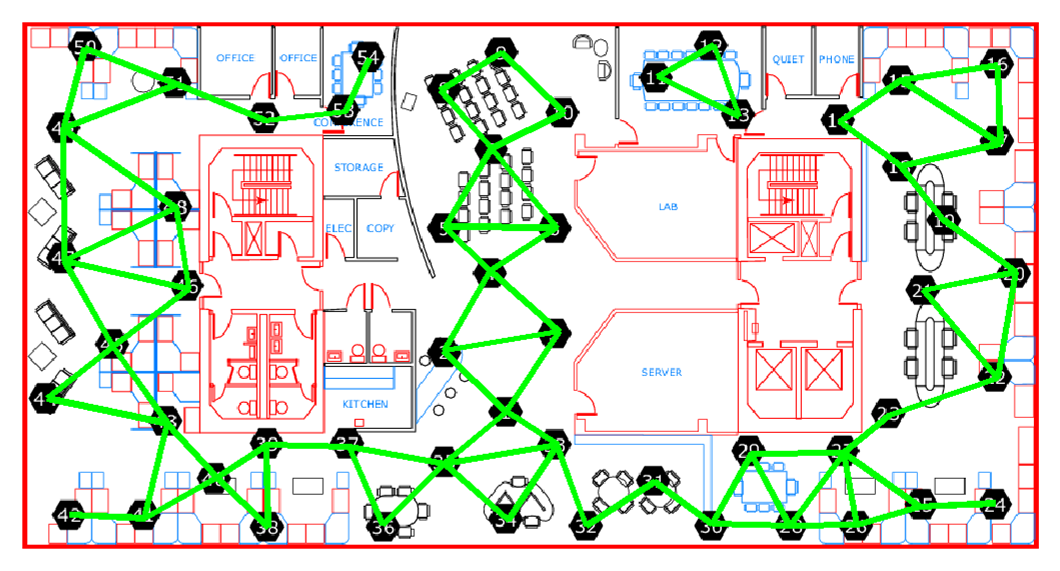
\includegraphics[width=0.30\textwidth]{expected.eps}
}
\hspace{0.1cm}
\subfigure[\hbox{Humidity: top 100 similar pairs}]{
	\label{fig:humidity_similarity}
	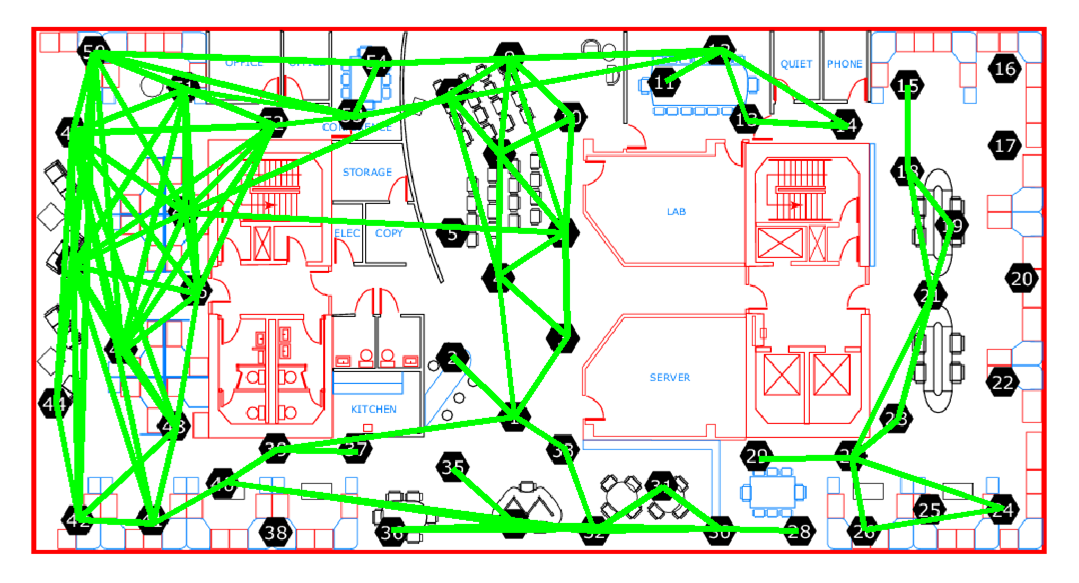
\includegraphics[width=0.30\textwidth]{Hum_similarity.eps}
}
\hspace{0.1cm}
\subfigure[\hbox{Light: top 100 similar pairs}]{
	\label{fig:light_similarity}
	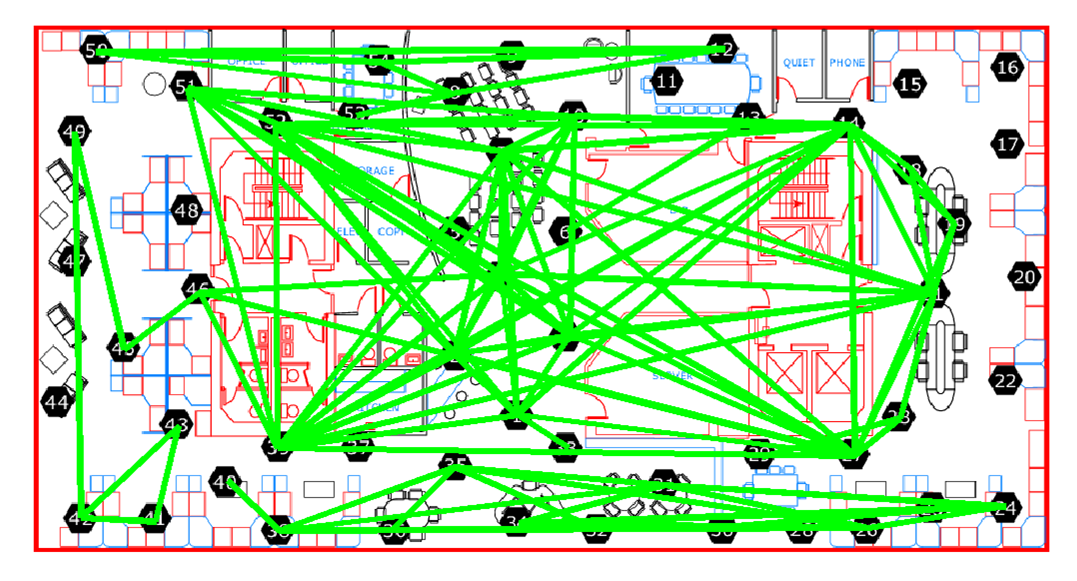
\includegraphics[width=0.30\textwidth]{Light_similarity.eps}
}
\vspace{-0.3cm}
\caption{Expected vs.~Actual Similarities}
\label{fig:similarity}
\vspace{-0.3cm}
\end{figure}


We also conduct an interesting experiment to see whether the correlations learned by TR-MF in random missing cases reflect our hypothesis of spatial correlation (i.e., Figure \ref{fig:expected_similarity}).
For the humidity and light data, we first use the TR-MF model to learn the latent factors of each sensor node given random missing under 85\% training data.
Based on the latent factors $\mathbf{q}$, we can then define the similarity between sensor nodes $n_i$ and $n_j$ as:
%\begin{equation*}
$\frac{q_{n_i}^T q_{n_j}}{max(||q_{n_i}||^2, ||q_{n_j}||^2)},$
%\end{equation*}
%and we get the similarity graph as Figure \ref{fig:similarity}.

Then we identify the top 100 similar pairs and draw a line between each of them on the floor plan.
We can see that the manually hypothesized spatial correlation plot Figure \ref{fig:expected_similarity} is more similar to the one learned from humidity data (Figure \ref{fig:humidity_similarity}) than to the one learned from light data (Figure \ref{fig:light_similarity}).
This experiment shows two interesting insights.
First, the manually-crafted spatial correlations do not necessary reflect the true correlations between sensor signals, because they might have not yet considered other factors such as barriers or long-distance correlations. 
%those described in the example of Figure \ref{fig:example_home_floorplan}.
Second, if the human knowledge of spatial correlation does to some extent reflect the true correlations between sensors, incorporating them in scenarios with limited information can be helpful (e.g., the humidity imputation for the consecutive missing patten in Table \ref{table:spatial} improves with spatial information); otherwise it is useless (e.g., no improvement on the light imputation for the consecutive missing pattern in Table \ref{table:spatial}).
